%You can leave alone everything before Line 79.
\documentclass{article}
\usepackage{url,amsfonts, amsmath, amssymb, amsthm,color, enumerate}
% Page layout
\setlength{\textheight}{8.75in}
\setlength{\columnsep}{2.0pc}
\setlength{\textwidth}{6.5in}
\setlength{\topmargin}{0in}
\setlength{\headheight}{0.0in}
\setlength{\headsep}{0.0in}
\setlength{\oddsidemargin}{0in}
\setlength{\evensidemargin}{0in}
\setlength{\parindent}{1pc}
\newcommand{\shortbar}{\begin{center}\rule{5ex}{0.1pt}\end{center}}
%\renewcommand{\baselinestretch}{1.1}
% Macros for course info
\newcommand{\courseNumber}{ME 552}
\newcommand{\courseTitle}{Mechatronics}
\newcommand{\semester}{Fall 2012}
\newcommand{\xxx}[1]{\textcolor{red}{#1}}
% Theorem-like structures are numbered within SECTION units
\theoremstyle{plain}
\newtheorem{theorem}{Theorem}[section]
\newtheorem{lemma}[theorem]{Lemma}
\newtheorem{corollary}[theorem]{Corollary}
\newtheorem{proposition}[theorem]{Proposition}
\newtheorem{statement}[theorem]{Statement}
\newtheorem{conjecture}[theorem]{Conjecture}
\newtheorem{fact}{Fact}
%definition style
\theoremstyle{definition}
\newtheorem{definition}[theorem]{Definition}
\newtheorem{example}{Example}
\newtheorem{problem}[theorem]{Problem}
\newtheorem{exercise}{Exercise}
\newtheorem{algorithm}{Algorithm}
%remark style
\theoremstyle{remark}
\newtheorem{remark}[theorem]{Remark}
\newtheorem{reduction}[theorem]{Reduction}
%\newtheorem{question}[theorem]{Question}
\newtheorem{question}{Question}
%\newtheorem{claim}[theorem]{Claim}
%
% Proof-making commands and environments
\newcommand{\beginproof}{\medskip\noindent{\bf Proof.~}}
\newcommand{\beginproofof}[1]{\medskip\noindent{\bf Proof of #1.~}}
\newcommand{\finishproof}{\hspace{0.2ex}\rule{1ex}{1ex}}
\newenvironment{solution}[1]{\medskip\noindent{\bf Problem #1.~}}{\shortbar}

%====header======
\newcommand{\solutions}[4]{
%\renewcommand{\thetheorem}{{#2}.\arabic{theorem}}
\vspace{-2ex}
\begin{center}
{\small  \courseNumber, \courseTitle
\hfill {\Large \bf {#1} }\\
\semester, University of Michigan, Ann Arbor \hfill
{\em Date: #3}}\\
\vspace{-1ex}
\hrulefill\\
\vspace{4ex}
{\LARGE Lab Assignment #2}\\
\vspace{2ex}
\end{center}
\begin{trivlist}
\item \textsc{Team members:\\} {#4}
\end{trivlist}
\noindent
\shortbar
\vspace{3ex}
}
% math macros
\newcommand{\defeq}{\stackrel{\textrm{def}}{=}}
\newcommand{\Prob}{\textrm{Prob}}
%==
\usepackage{graphicx}
\begin{document}
%%%%%%%%%%%%%%%%%%%%%%%%%%%%%%%%%%%%%%%%%%%%%%%%%
%\solutions{Your name}{Problem Set Number}{Date of preparation}{Collaborators}{Prover}{Verifiers}
\solutions{}{1}{\today}{Shiva Ghose, @gshiva\\ John Peterson, @jrpeters\\ Wenjian Bai, @baiwenji}
%%%%%%%%%%%%%%%%%%%%%%%%%%%%%%%%%%%%%%%%%%%%%%%%%
%\renewcommand{\theproblem}{\arabic{problem}} 
%%%%%%%%%%%%%%%%%%%%%%%%%%%%%%%%%%%%%%%%%%%%%%%%%
%
% Begin the solution for each problem by
% \begin{solution}{Problem Number} and ends it with \end{solution}
%
% the solution for Problem 

\section*{Question 1}



\section*{Question 2}

\subsection*{a}

\begin{figure}[h]
\begin{center}
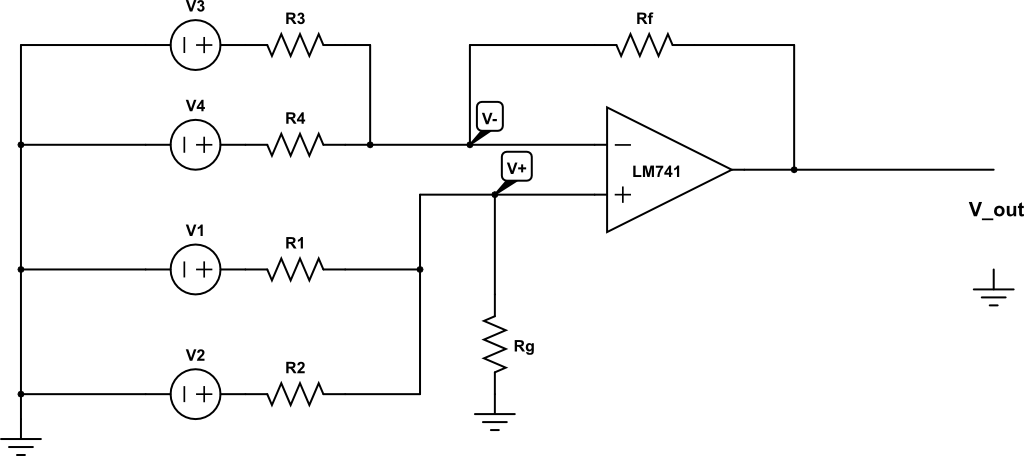
\includegraphics[width=10cm]{q2_circuitDiagram.png}
\end{center}
\caption{The required circuit diagram for question 2.}
\label{q2_a}
\end{figure}


\subsection*{b}
Circuit analysis:\\

At the non-inverting terminal, we effectively have a circuit represented by figure \ref{q2_b1}. We can use Kirchoff's voltage law along with the superposition theorem, we see:
\begin{figure}[h]
\begin{center}
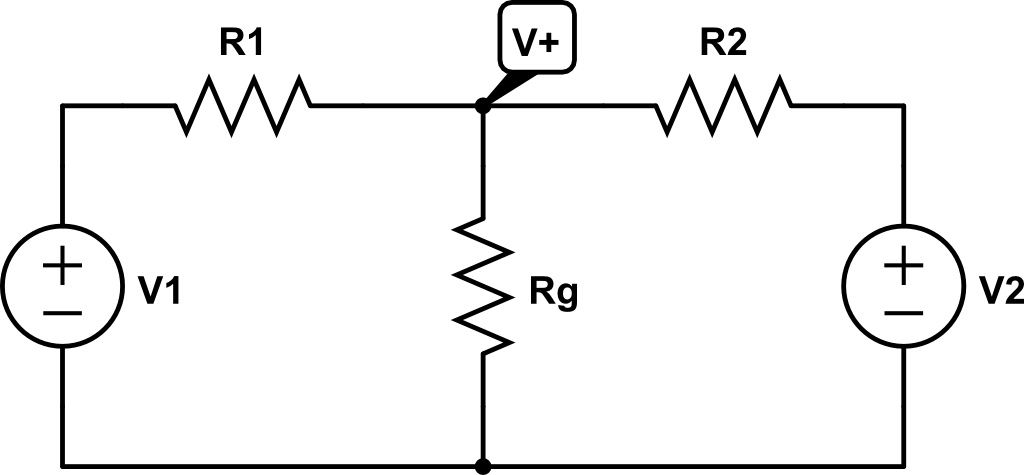
\includegraphics[width=6cm]{lab1_q2_kvl1.png}
\end{center}
\caption{Equivalent circuit at the non-inverting terminal}
\label{q2_b1}
\end{figure}

$$\text{Voltage at $V^+$ due to $V_1$, $V^+_1$, is given by:}$$
$$V^+_1 = \frac{\frac{R_2 R_g}{R_2+R_g}}{R_1 + \frac{R_2 R_g}{R_2+R_g}}\ V_1$$
$$\therefore V^+_1 = \Big(\frac{1}{\frac{R_1}{R_g} + \frac{R_1}{R_2} + 1}\Big) \ V_1$$

$$\text{Similarly, voltage at $V^+$ due to $V_2$, $V^+_2$, is given by:}$$
$$V^+_2 = \frac{\frac{R_1 R_g}{R_1+R_g}}{R_2 + \frac{R_1 R_g}{R_1+R_g}}\ V_2$$
$$\therefore  V^+_2 = \frac{1}{\frac{R_2}{R_g} + \frac{R_2}{R_1} + 1} \ V_2$$

$$\text{Using the superposition theorem to recombine the values, we find that $V+$ is given by:}$$
$$V^+ = V^+_1 + V^+_2 $$
$$V^+ = \frac{1}{\frac{R_1}{R_g} + \frac{R_1}{R_2} + 1} \ V_1 + \frac{1}{\frac{R_2}{R_g} + \frac{R_2}{R_1} + 1} \ V_2 $$

We can now move on to the inverting terminal of the op-amp. The corresponding equivalent circuit is shown in figure \ref{q2_b2}.  Analyzing this circuit, we see that:
\begin{figure}[h]
\begin{center}
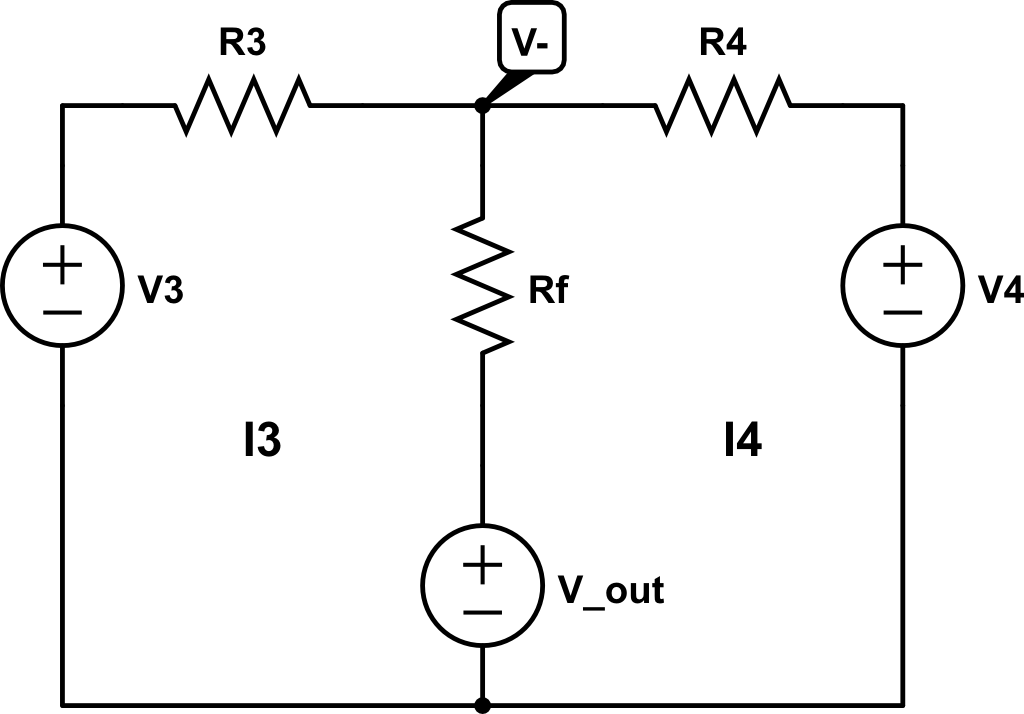
\includegraphics[width=6cm]{lab1_q2_kvl2.png}
\end{center}
\caption{Equivalent circuit at the non-inverting terminal}
\label{q2_b2}
\end{figure}
$$I_3R_3 = V_3 - V^-$$
$$I_4R_4 = V_4 - V^-$$
$$V^- - V_{out} = (I_3 + I_4)R_f $$
$$\text{Substituting from the above equations, we get:}$$
$$ V^- - V_{out} = \Big( \frac{ V_3 - V^-}{R_3} + \frac{ V_4 - V^-}{R_4}\Big) \ R_f$$
$$\text{Reordering the terms, we get:}$$
$$V_{out} =V^- -  \Big( \frac{ V_3 - V^-}{R_3} + \frac{ V_4 - V^-}{R_4}\Big) \ R_f $$
$$\implies V_{out} =V^- \Big( \frac{R_f}{R_3} + \frac{ R_f}{R_4} + 1\Big) - \Big( \frac{R_f}{R_3}\Big)V_3 - \Big( \frac{ R_f}{R_4}\Big)V_4$$

We also know that for an ideal op-amp, $V^+ = V^-$, hence we get:
$$ V_{out} = \Big( \frac{R_f}{R_3} + \frac{ R_f}{R_4} + 1\Big) \Big( \frac{1}{\frac{R_1}{R_g} + \frac{R_1}{R_2} + 1}\Big) V_1 + \Big( \frac{R_f}{R_3} + \frac{ R_f}{R_4} + 1\Big) \Big( \frac{1}{\frac{R_2}{R_g} + \frac{R_2}{R_1} + 1} \Big) V_2 - \Big( \frac{R_f}{R_3}\Big)V_3 - \Big( \frac{ R_f}{R_4}\Big)V_4$$

This is equation is the mathematical representation of the required problem which was; $V_{out} = a_1V_1 + a_2 V_2 - a_3 V_3 - a_4 V_4$, i.e. :
$$a_1 =  \Big( \frac{R_f}{R_3} + \frac{ R_f}{R_4} + 1\Big) \Big( \frac{1}{\frac{R_1}{R_g} + \frac{R_1}{R_2} + 1}\Big)$$
$$a_2 =  \Big( \frac{R_f}{R_3} + \frac{ R_f}{R_4} + 1\Big) \Big( \frac{1}{\frac{R_2}{R_g} + \frac{R_2}{R_1} + 1} \Big) $$
$$a_3 = \Big( \frac{R_f}{R_3}\Big)$$
$$a_4 = \Big( \frac{ R_f}{R_4}\Big)$$

\subsection*{c}

\end{document}


\def\therefore{\boldsymbol{\text{ }
\leavevmode
\lower0.4ex\hbox{$\cdot$}
\kern-.5em\raise0.7ex\hbox{$\cdot$}
\kern-0.55em\lower0.4ex\hbox{$\cdot$}
\thinspace\text{ }}}
